\documentclass{article}
\usepackage{tikz}
\usetikzlibrary{positioning}
\usepackage{listings}
\lstset{
  basicstyle=\ttfamily\small,
  breaklines=true,
  frame=single
}

\title{MPI File Transfer System}
\author{Nguyen Viet Khoa}
\date{\today}

\begin{document}

\maketitle

\section{Why the Chosen MPI Implementation}
I chose mpi4py, the Python bindings for MPI, because it integrates seamlessly with existing Python code from the original TCP system. It is easy to install and use, supports high-level operations such as send/recv, and works with standard MPI backends, including OpenMPI. This avoids rewriting in lower-level languages like C++, making the upgrade straightforward while maintaining portability across clusters.

\section{Design of the MPI Service}
The MPI service uses a single-program multiple-data (SPMD) model where all processes run the same script. Rank 0 acts as the server, reading the file and sending it in chunks to Rank 1 (the client), which receives and saves the data. Communication uses MPI send/recv for simplicity. File size is sent first to handle reception, and chunks prevent message overflow for large files.

\begin{figure}[h]
\centering
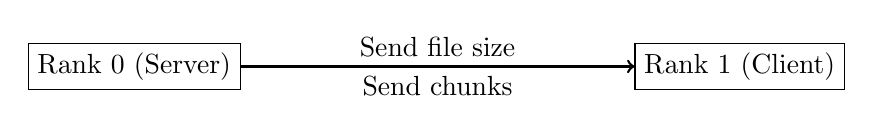
\begin{tikzpicture}
  \node[draw, rectangle] (rank0) {Rank 0 (Server)};
  \node[draw, rectangle, right=of rank0, xshift=4cm] (rank1) {Rank 1 (Client)};
  \draw[->, thick] (rank0) -- node[above] {Send file size} (rank1);
  \draw[->, thick] (rank0) -- node[midway, below] {Send chunks} (rank1);
\end{tikzpicture}
\caption{MPI Service Design}
\label{fig:design}
\end{figure}

\section{Organization of the System}
The system is organized in a new directory called \texttt{MPI}, copied from the original TCP implementation. It contains:
\begin{itemize}
  \item \texttt{mpi\_file\_transfer.py}: The main MPI script handling both server and client logic based on rank.
  \item Files to transfer (e.g., \texttt{example.txt}) placed in the directory accessible by rank 0.
\end{itemize}
No separate server/client files are needed, as MPI handles process differentiation. Run with \texttt{mpirun -np 2 python mpi\_file\_transfer.py <filename>}.

\begin{figure}[h]
\centering
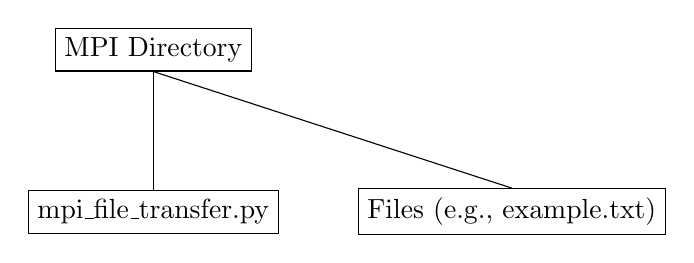
\begin{tikzpicture}
  \node[draw, rectangle] (mpi) {MPI Directory};
  \node[draw, below=of mpi, yshift=-0.5cm] (script) {mpi\_file\_transfer.py};
  \node[draw, right=of script] (files) {Files (e.g., example.txt)};
  \draw (mpi.south) -- (script.north);
  \draw (mpi.south) -- (files.north);
\end{tikzpicture}
\caption{System Organization}
\label{fig:organization}
\end{figure}

\section{Implementation of the File Transfer}
The file transfer uses MPI's \texttt{send} and \texttt{recv} for data exchange. The server (rank 0) reads the file, sends its size, then chunks the data. The client (rank 1) receives the size, then accumulates chunks and writes to a new file. Here's a code snippet:

\begin{lstlisting}[language=Python, caption=Core Implementation Snippet]
if rank == 0:  # Server
    with open(filename, 'rb') as f:
        file_data = f.read()
    file_size = len(file_data)
    comm.send(file_size, dest=1)
    for i in range(0, file_size, CHUNK_SIZE):
        chunk = file_data[i:i + CHUNK_SIZE]
        comm.send(chunk, dest=1)

elif rank == 1:  # Client
    file_size = comm.recv(source=0)
    received_data = b''
    remaining = file_size
    while remaining > 0:
        chunk = comm.recv(source=0)
        received_data += chunk
        remaining -= len(chunk)
    with open(received_filename, 'wb') as f:
        f.write(received_data)
\end{lstlisting}

\section{Who Does What}
\begin{itemize}
  \item \textbf{Rank 0 (Server)}: Checks arguments, reads the local file, sends the file size, chunks, and sends the data via MPI. Handles errors like file not found by sending a signal (-1).
  \item \textbf{Rank 1 (Client)}: Receives the file size, accumulates chunks until complete, and writes the data to a new local file. Exits on error signals.
\end{itemize}

\end{document}